% 图 13.4 —— 由 `checks/emit_hand.py` 自动拼出（probe 精测 + prims2 图元分解）
%%
% ⚠ 这是**稿子不是成品**：跑 `checks/checkhand.py 13.4` 看指标 + 看叠合图。
%%
%% ⚠ 待核：
%   · 本图 probe 报出阴影族 1 个 —— **本脚本不生成阴影**（要照原书手写）；prims2 的 strokes 里可能含阴影线，核对时留意别画重
%   · 可疑字形 1 项（空心圈 ⊙ 常被认成字母 o）—— 见文件末
%%
\documentclass[12pt]{standalone}
\usepackage{fontspec}
\setsansfont{Arial}
\newfontfamily\mfallback{DejaVu Sans}
\usepackage{tikz}
\begin{document}
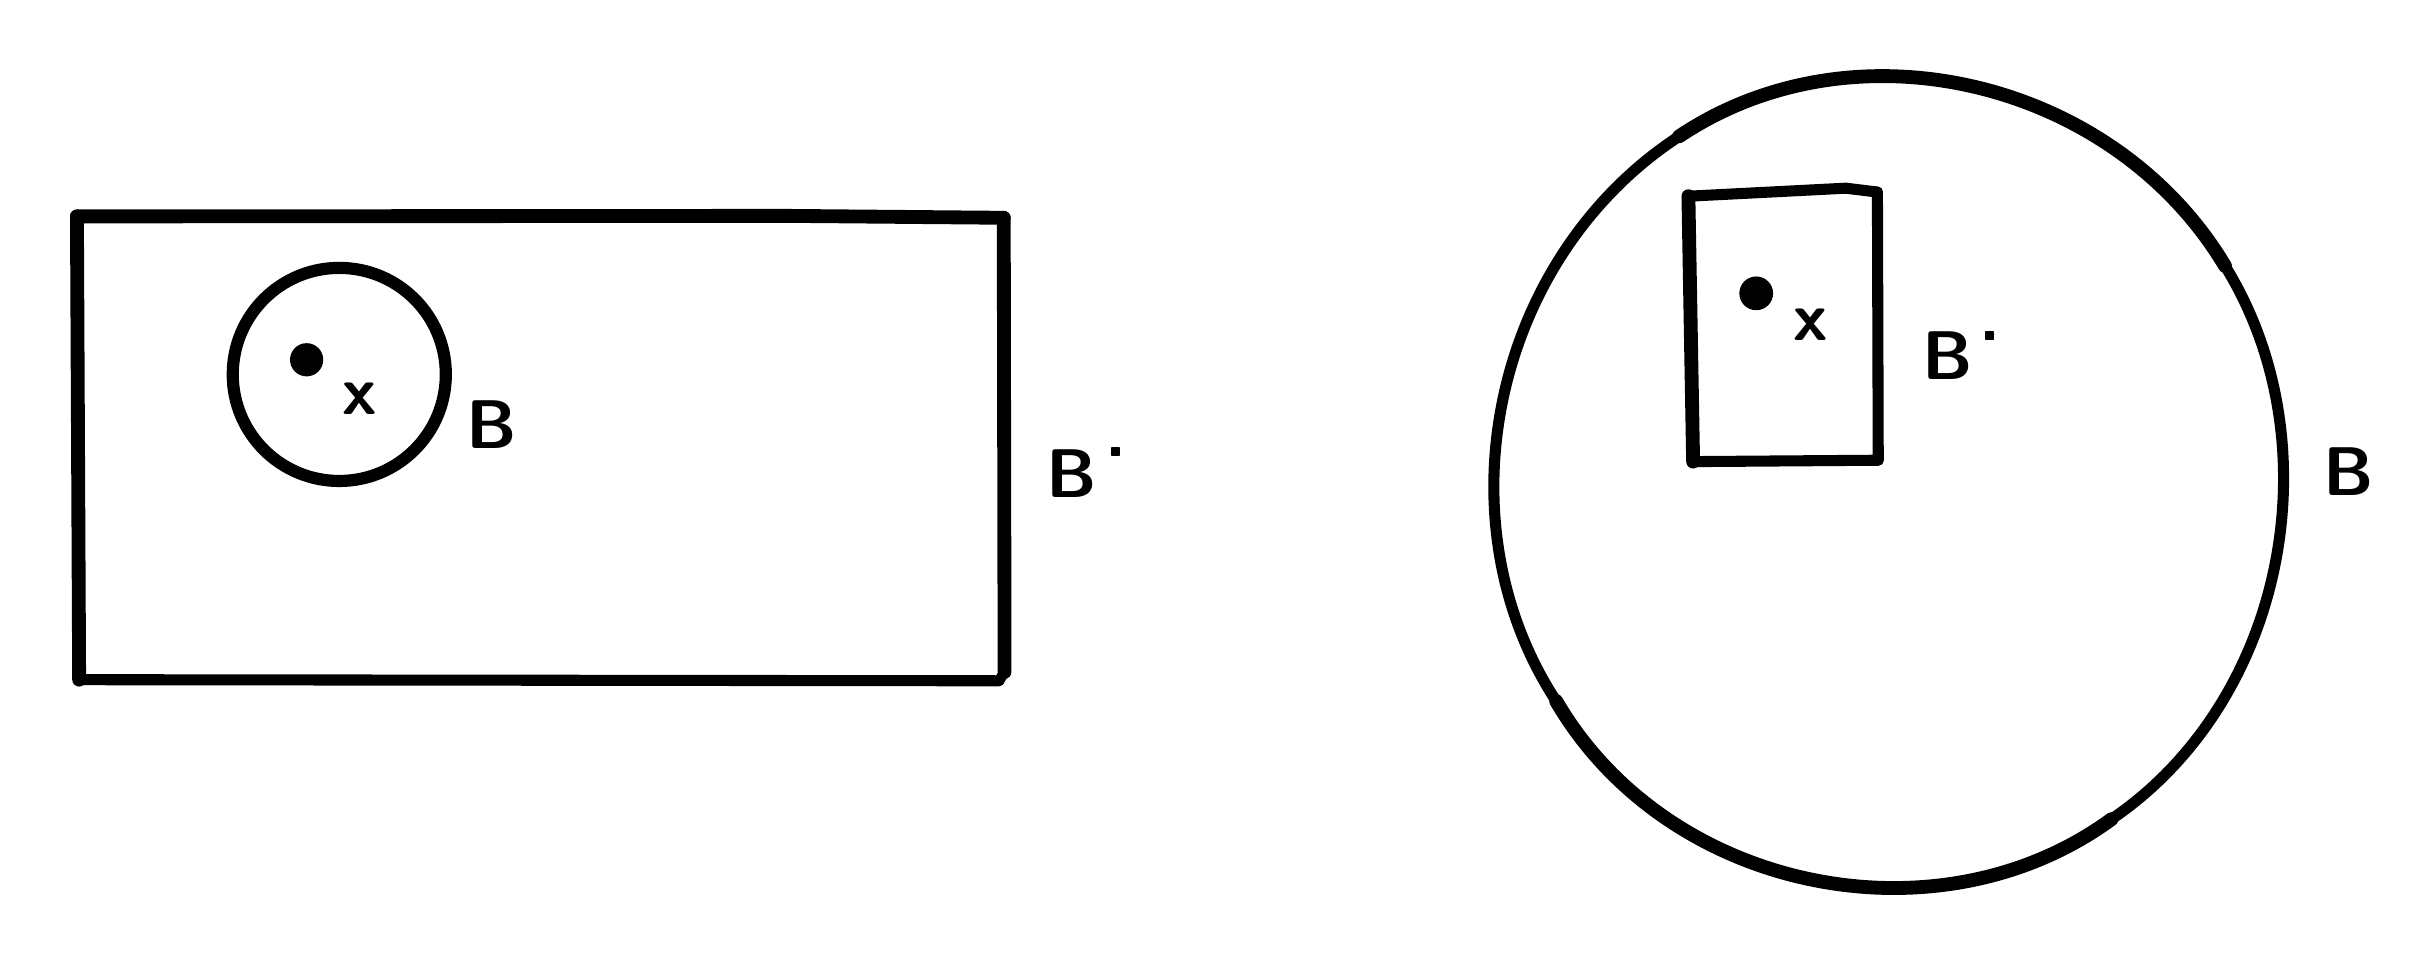
\begin{tikzpicture}[x=1pt, y=-1pt, line width=4.4pt, line cap=round, line join=round]

  %% ════ 填充区（prims2 的 fills）════

  %% ════ 直线段（prims2 的 strokes）════
  \draw[line width=5.0pt] (274.0,68.0) -- (17.8,68.2);
  \draw[line width=5.0pt] (17.8,68.2) -- (18.6,235.6);
  \draw[line width=4.0pt] (18.6,235.6) -- (351.0,236.0);
  \draw[line width=3.8pt] (351.0,236.0) -- (353.0,232.8);
  \draw[line width=5.0pt] (353.0,232.8) -- (352.7,68.7);
  \draw[line width=5.0pt] (352.7,68.7) -- (274.0,68.0);
  \draw[line width=4.0pt] (657.0,58.0) -- (600.1,60.9);
  \draw[line width=5.0pt] (600.1,60.9) -- (601.8,156.8);
  \draw[line width=4.0pt] (601.8,156.8) -- (668.7,156.3);
  \draw[line width=4.0pt] (668.7,156.3) -- (668.4,59.4);
  \draw[line width=4.0pt] (668.4,59.4) -- (657.0,58.0);

  %% ════ 曲线（prims2 的 curves —— 三段式，坐标同为 (y,x)）════
  \draw[line width=4.0pt] (753.0,286.0) .. controls (816.5,242.8) and (833.5,149.8) .. (794.0,86.1);
  \draw[line width=5.0pt] (794.0,86.1) .. controls (754.2,19.5) and (660.8,-3.7) .. (596.7,39.3);
  \draw[line width=4.0pt] (596.7,39.3) .. controls (529.8,83.0) and (509.4,177.7) .. (552.3,243.3);
  \draw[line width=5.0pt] (552.3,243.3) .. controls (592.4,312.2) and (690.1,332.0) .. (753.0,286.0);

  %% ════ 圆 / 椭圆（probe 精测）════
  \draw (112.6,125.3) circle (38.5);

  %% ════ 实心点 ════
  \fill (624.6,96.0) circle (6.1);
  \fill (100.8,120.0) circle (6.0);

  %% ════ 标签（probe 直接给的 \node 行）════
  %% ⚠ 全部补了 fill=white：文字在最上层，否则与曲线交叉干扰
     \node[anchor=center,inner sep=0pt,fill=white,font=\fontsize{28.3}{35.4}\selectfont] at (644.4,107.4) {\textsf{\textbf{\textit{x}}}};   % box(636,97,15,17)
     \node[anchor=center,inner sep=0pt,fill=white,font=\fontsize{30.3}{37.9}\selectfont] at (693.8,118.5) {\textsf{\textbf{\textit{B}}}};   % box(682,107,20,22)
     \node[anchor=center,inner sep=0pt,fill=white,font=\fontsize{42.4}{53.0}\selectfont] at (709.2,111.4) {\textsf{\textbf{.}}};   % box(704,107,4,8)
     \node[anchor=center,inner sep=0pt,fill=white,font=\fontsize{30.1}{37.6}\selectfont] at (120.0,134.0) {\textsf{\textbf{\textit{x}}}};   % box(111,123,16,18)
     \node[anchor=center,inner sep=0pt,fill=white,font=\fontsize{30.3}{37.9}\selectfont] at (167.8,143.5) {\textsf{\textbf{\textit{B}}}};   % box(156,132,20,22)
     \node[anchor=center,inner sep=0pt,fill=white,font=\fontsize{42.4}{53.0}\selectfont] at (393.2,153.4) {\textsf{\textbf{.}}};   % box(388,149,4,8)
     \node[anchor=center,inner sep=0pt,fill=white,font=\fontsize{30.3}{37.9}\selectfont] at (838.8,160.5) {\textsf{\textbf{\textit{B}}}};   % box(827,149,20,22)
     \node[anchor=center,inner sep=0pt,fill=white,font=\fontsize{30.4}{38.0}\selectfont] at (377.3,161.0) {\textsf{\textbf{\textit{B}}}};   % box(365,150,21,21)

  % 钉死画布：否则超出的图元/控制点会把页面撑大，1:1 回比就失准
  \pgfresetboundingbox
  \path[use as bounding box] (0,0) rectangle (858,325);
\end{tikzpicture}
\end{document}

% ⚠ 待核清单（probe 拿不准，人眼过一遍）：
%   · 未识别/跳过：⑤ 跳过/未识别的字形
